\chapter{Basics}
Everything necessary to understand the implementation as well as anything which is done beforehand, will come up here

In the following, all concepts, technologies and required backgrounds for understanding this thesis are explained. 


\section{Data}
Well talk about data a bit. Where does it come from? How is it structured? What kind of attributes? What even are attributes?

Since ancient times, humans have recorded data. Recording the ins and outs of available resources was one of the driving factors behind the conceptualization of writing. (TODO: Check sources of the beer brewing video series)
With the introduction of computers the amounts of gathered data have grown drastically. Vast amounts of data are gathered across all aspects of life.

\subsection{Types of Data}
Even though data comes from a huge variety of sources and can express a plethora of things, there are only four different types of data. They are split into equal pairs. Two types of categorical data and two types of numerical data. In the following each of the types of data will be explained.

\subsubsection{Categorical}
What is categorical data? Nominal and ordinal data

Categorical or qualitative data is information collected in groups. It is often of descriptive nature. Whilst the values can be represented in numbers, they do not allow for arithmetic operations.
There are two types of categorical data. Nominal and ordinal data.

\paragraph{Nominal}
data is mostly descriptive in nature. They are independent and have no inherit order. Examples are 'Country', 'Color', 'Brand'.

\paragraph{Ordinal}
data is mostly similar to nominal data. Yet the data does have some sort of internal order. For example different dates each describe a day, but one day also comes after another.

\subsubsection{Numeric}
What is numeric data? Continuous and Discrete

Numeric or quantitative data is all data expressed in numbers, where numbers do not represent categories. It allows for arithmetical operations and can be split into Discrete and Continuous data.

\paragraph{Discrete}
data can only take certain defined values. This usually means whole numbers to represent things that can not be split up further. Like the 'Number of Refugees' or 'Tickets sold'. Discrete data is countable.

\paragraph{Continuous}
data can be measured. It can have any real number as value. Therefore fractions are possible as well. For example when measuring the temperature, or the length or weight of an object.

\subsection{Datasets}
What are our datasets about? Where do they come from?

Datasets are a collection of several data-points. each of these data-points is made up of different attributes. Each attribute corresponds to a specific data-type.

In this thesis, two data-sets are used. They are both from UNHCR\cite{unhcr}. The first data-set contains information about the total number of refugees per country\cite{unhcr_rpc}. The second dataset is about the total cumulative total amount of refugees per day\cite{unhcr_rpd}. Both data-sets are in the JSON format.

\subsubsection{Preprocessing}
What is done in preprocessing? Python script which removes all excess / maybe do that in JS as well..?

As both of the used data-sets have a lot of 'unnecessary' information, they are both preprocessed. In both cases the data-sets are read and the valuable information extracted and saved in the csv format. Both of the newly created csv files have two columns and one header row. The resulting csv of the refugees per country dataset, contains the two columns of country and refugees. The other resulting csv contains a column for the date and one for the cumulative refugees.
The data-set about the refugees per country can also easily be converted into using percentages. After adding up the total amount of refugees from each data-point, one can convert the absolute number of refugees into percent.

\subsubsection{Data Types}
Which data types can be found in our data-sets? Where?

The two chosen data-sets already cover most of the data-types. The refugees per country dataset contains two attributes per data-point. The country is a categorical attribute. The number of refugees is discrete. When converting this data-set into using percentages, the percentage of refugees becomes a continuous attribute. The In the refugees per date data-set, the amount of refugees is still a discrete attribute. The date itself is an ordinal attribute though. As one day clearly comes before and after another day.

Choosing data-sets which cover all types of data-types was an important consideration. Different data-types can have different ways of representation, as well as different ways of implementation on the programming side of things.


\subsection{Data Visualization}
What is it? Where is it? Why is it important?

Data visualization is the process of turning data into graphical representations. As the vast amounts of data which are gathered in charts and databases are often hard to comprehend with the human mind and might require a big amounts of space to directly represent, it is often desired to turn these data-sets into a more easily understandable formats. Therefore data is turned into diagrams. We constantly come across the results of data visualization in everyday life. They can be commonly found across all kinds of news sources, but also in reports, information campaigns or as part of user-interfaces in machinery or control systems. 


\section{Diagrams}
What diagrams exists? Which are the most common? What possibilities do they offer for encoding data? Which considerations for readability? Why do some diagrams not make as much sense? Which considerations where made for fulfilling the showcase requirements?

Diagrams exists in many different shapes and sizes. There are many factors which should be taken into consideration when deciding which diagram to choose. There are usually many ways to represent the desired data. Some of the most common diagrams include bar-charts, pie-charts and scatter-plots (TODO: Find source (lel))

All diagrams use a combination of marks and channels to encode data. Marks usually depend on the type of data. They are usually single points, lines or areas in a diagram. Channels depend on the singular data-points and influence the marks. The most common channels are position, color and size. It is important to note, that not all channels work with all data-types.

\begin{figure}
    \label{fig:bar-chart}
    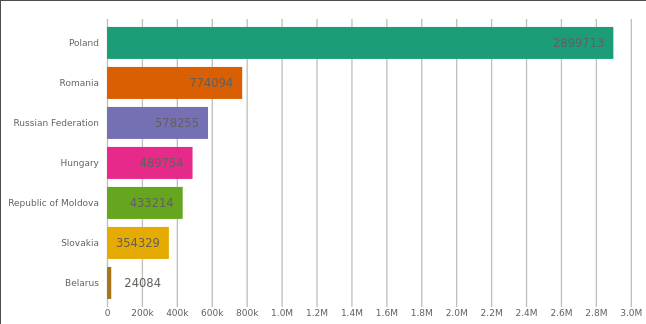
\includegraphics[width=\linewidth]{bar-chart.png}
    \caption[bar-chart]{This is a bar-chart (TODO: which needs a frame..?)}
\end{figure}

\begin{figure}
    \label{fig:donut-chart}
    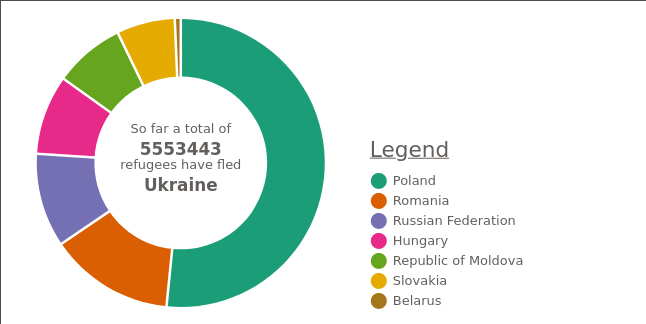
\includegraphics[width=\linewidth]{donut-chart.png}
    \caption[donut-chart]{This is a donut-chart (TODO: which needs a frame..?)}
\end{figure}

To understand this more easily, we can look at diagram \ref{fig:bar-chart}. This diagram uses lines as marks. The y-position, as well as the hue, are both used to encodes the same categorical attribute. The area/size encodes a discrete attribute. The donut chart(\ref{fig:donut-chart}) instead used areas as marks. Their size encodes a discrete, whilst the hue encodes a categorical attribute.

Different combinations of marks and channels can influence the readability and the correctness of how the represented data is comprehended \cite{heer2010crowdsourcing} \cite{mackinlay1986automating}.


\section{D3.js}
This is all about d3. What is it? Where does it come from? What is it used for? Who uses it? Why should it be used? How does it work? Enter, update and exit pattern. Something about the modular structure of D3 as well. Might be worth mentioning "observables" as well.

"D3.js is a JavaScript library for manipulating documents based on data. D3 helps you bring data to life using HTML, SVG, and CSS."\cite{d3js}. The name D3 is short for data-driven documents. The D3 library was originally created by Mike Bostock and is published under the BSD-3-Clause open-source license.

\subsection{How does it work?}
General functioning of D3.

"D3 allows you to bind arbitrary data to a Document Object Model (DOM), and then apply data-driven transformations to the document."\cite{d3js}. There are three main concepts that make up the core of D3. Selections, data joins and the general update pattern. Importing the d3 library into a project allows access to the \verb|d3| namespace.

\subsubsection{Selections}
What are they? Why are they useful?

All operations in D3 run on an arbitrary collection of nodes these collections of nodes are called selections. There are two functions in D3 to create a new selection: \verb|d3.select("selector")| and \verb|d3.selectAll("selector")|. Both functions require a selector for identifying the appropriate elements. The selectors are defined in the W3C Selectors API\cite{w3c_selectors_api}. It is possible to directly access the DOM elements as the selections are only collections of nodes. But there are also many predefined functions for modifying the nodes properties. This includes the modification of attributes and styles, as well as event handling. Selections can also be extended or shrunken by adding or removing nodes, or by combining multiple selections.

\subsubsection{Data Joins}
What are they and why are they important?

Data joins are a key feature of D3. They link up a data-point to a specific DOM element. To create a data-join, one has to call the \verb|.data(dataset)| function on a selection. It takes a dataset, an array of data-points, as parameter. This will bind the data elements to the nodes in the selection. When we want to create diagrams which can respond to data changes over time, it is usually also a good idea to specify a identifier function for the data-points. As the default identifier corresponds to the index of the data-point. This can lead to unexpected behavior when the dataset is modified. It is not important for the number of data-points to match up with the number of nodes in the selection. This is taken care of through the general update pattern.

\subsubsection{General Update Pattern}
What is it? What can it do? Describe data joins and dom element links.

The general update pattern is another core concept of D3. Every time a data join is created or updated, it comes into play. There are three possible cases that can happen, when a data join is invoked. The first case, which usually happens as the data join is first created, is, that there are more data-points than nodes. In this case, all the data-points without a linked node are called the enter selection. The second case is about data-points which already have a linked DOM element. They make up the update selection. The last case , where a data-point which was already linked to a DOM element has been removed, is called the exit selection. For each three of the resulting sub-selections, we can define the behavior. For the entry selection, we usually want to create a new DOM element to represent the data-point. When the goal is to create only static representations, it is even enough to only implement the entry functionality. If we want to allow for data to change over time, we probably also want to implement the update and exit selections behaviors.


\subsubsection{Modules}
The way D3 is split up into modules, the core package and what kind of extensions are there.
